\documentclass[10pt, conference, compsocconf]{IEEEtran}

\ifCLASSINFOpdf

\else

\fi

\usepackage{hyperref}
\usepackage{amsmath}
\usepackage{amssymb}
\usepackage{hhline} % easy to manage table borders
\usepackage{colortbl} % colored cells in tables
\usepackage{multirow}
\usepackage{enumerate}
\usepackage{slashbox} % cell with slash inside
\usepackage{makeidx}  % allows index generation
\usepackage[utf8]{inputenc}
\usepackage{graphicx}

\newtheorem{definition}{Definition}
\newtheorem{example}{Example}

\def\sectionautorefname{Section}
\def\subsectionautorefname{Section}


% correct bad hyphenation here
\hyphenation{op-tical net-works semi-conduc-tor}


\begin{document}

% paper title
% can use linebreaks \\ within to get better formatting as desired
\title{Pharmer -- Semantic Authoring of Medical Prescriptions}
%\title{Pharmer: A platform for health care providers to use linked open data in e-prescriptions}


% author names and affiliations
% use a multiple column layout for up to two different
% affiliations

\author{\IEEEauthorblockN{Ali Khalili}
\IEEEauthorblockA{Faculty of Computer Science\\
University of Leipzig\\
Leipzig, Germany\\
khalili@informatik.uni-leipzig.de}
\and
\IEEEauthorblockN{Bita Sedaghati}
\IEEEauthorblockA{Institute of Pharmacy\\
University of Leipzig\\
Leipzig, Germany\\
bita.sedaghati@uni-leipzig.de}
}


% make the title area
\maketitle

\begin{abstract}
The abstract goes here. DO NOT USE SPECIAL CHARACTERS, SYMBOLS, OR MATH IN YOUR TITLE OR ABSTRACT.

\end{abstract}

\begin{IEEEkeywords}
component; formatting; style; styling;

\end{IEEEkeywords}


\IEEEpeerreviewmaketitle



\section{Introduction}
This is a test \cite{Khalili2012}.

\section{Semantic Content Authoring}
\label{sec:sca}

\section{E-Prescriptions}
E-prescriptions are computer-generated prescriptions utilized by healthcare providers.
They perform an important role in improving the quality of patient care.
E-prescriber electronically send an accurate, error-free and understandable prescription directly to a pharmacy from the point-of-care.
While even nowadays paper prescription are commonly used, electronic prescription has offered several advantages.
Improved confidentiality and security of health information, better clarity and communication among health care providers as well as rapid information exchange are part of arguments for spreading this systems.
Reduction in medication error and decline in adverse drug events are more highlighted consequences of e-prescribing.
During the recent years has been spreading rapidly.To illustrate, the Australian government started launching of e-prescription from 1 March 2007.

\section{Semantic Authoring of Medical Prescriptions}

\section{Pharmer}
In \autoref{fig:lod}, you can see..
We discussed sth in \autoref{sec:sca}.

\subsection{Architecture}

\begin{figure}[tb]
	\centering
		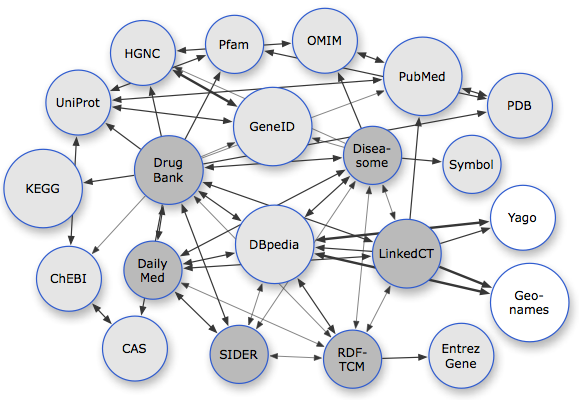
\includegraphics[width=1.0\columnwidth]{images/lod_cloud.png}
	\caption{Available datasets related to pharmaceutical research.}
	\label{fig:lod}
\end{figure}


\section{Conclusion}
The conclusion goes here. this is more of the conclusion

% conference papers do not normally have an appendix


% use section* for acknowledgement
\section*{Acknowledgment}


The authors would like to thank...
more thanks here

\bibliographystyle{IEEEtran}
% argument is your BibTeX string definitions and bibliography database(s)
\bibliography{refs}





% that's all folks
\end{document}


